
\documentclass[a4paper,12pt]{article}
\usepackage[utf8]{inputenc}
\usepackage[T1]{fontenc}
\usepackage[french]{babel}
\usepackage{csquotes}

\usepackage[left = 2cm, top = 2cm, right = 2cm, bottom = 2cm]{geometry}
\usepackage{physics}
\usepackage{siunitx}
% \qty should normally used to typeset SI quantities, but since it is already defined by the physics package, we need to use \SI
\sisetup{separate-uncertainty}
\sisetup{per-mode=fraction}
\usepackage{hyperref}
\usepackage{multirow}
\usepackage{svg}
\usepackage{pgfplots}
\usepgfplotslibrary{groupplots}
\pgfplotsset{compat=1.16}
\usepackage{biblatex} %Imports biblatex package
\addbibresource{bib.bib} %Import the bibliography file


\newcommand\nom[2][]{#1~\textsc{#2}}
\title{Rapport de stage de L3}
\author{\nom[Maurice]{Debray}}
\date{}

\begin{document}
\maketitle

\tableofcontents

\section{Introduction: Contexte du stage}

J'ai effectué mon stage au CEA au sein du Laboratoire de Développement et
d’Intégration de Systèmes de Contrôle (LDISC). Il est responsable du
développement des systèmes de contrôle-commande pour les
projets\footnote{Principalement des accélérateurs à particules, mais ils
participent à d'autres expériences comme ISEULT, un IRM de 11T.} du département
dont il fait partie (Département d'Ingénierie des Systèmes (DIS)). Mon tuteur était \nom{Rémi}{Nicole}.

Les expériences pour lesquels le LDISC est ammené à réaliser des développements
sont en général des expériences de long terme destinées à durer plusieurs
décennies avec du support et souvent des améliorations à apporter tout au long
de la vie des expériences. Ainsi, la conservation des environnements de
développement et des sources des projets (principalement les sources de projets
externes) est un enjeu crucial. En effet sur ces durées il arrive que des
programmes arrêtent d'être maintenus voire que les sources disparaissent.

Pour pallier à ce problème, le LDISC expérimente l'utilisation du gestionnaire
de paquets \texttt{Nix}. Ce dernier propose en effet de compiler les paquets dans un
environnement reproductible avec le minimum d'effet de bord (isolation). Pour
réaliser cela, il s'appuie sur une spécification stricte des dépendances par le
développeur via un language dédié (le langage \texttt{Nix}).


Le but de mon stage était multiple. Tout d'abord, il s'agissait de développer un
dépôt de paquets nix bien intégré avec l'intégration continue du Gitlab du CEA.\@
Ensuite, j'ai développé un outil permettant d'explorer l'arbre de dépendances
d'un paquet afin de permettre une conservation automatisé des sources des
paquets ainsi que des résultats de compilation afin d'augmenter la résilience de
l'infrastructure de contrôle commande du projet sur lequel Nix sera utilisé
(TITAN, un projet d'accélérateur à particule pour la direction des affaires militaires).

\section{Le fonctionnement de \emph{nix}}

Cette partie est une rapide introduction à nix. Pour un explication plus
complète, il convient de se référer à l'introduction du manuel de
\emph{nix}~\cite{nix}.

\subsection{Le langage \emph{nix}}

\emph{nix} est un gestionnaire de paquets et un langage. Le langage nix est un
langage fonctionnel, pure (ou presque) et parresseux.

La principale fonction avec effet de bord est la fonction \texttt{derivation} qui est
aussi le coeur du langage. Cette fonction (en plus de renvoyer un objet appelé
\emph{dérivation}) crée un fichier \texttt{.drv} dans le store lors de son
évaluation. Les fichiers \texttt{.drv} décrivent comment compiler un paquet
(dépendances nécessaires pour la compilation, commande à executer, shell à
utiliser, etc\dots).

\subsection{Le store}

Le programme \emph{nix} utilise un magasin appelé \emph{store}. Il est composé d'un
dossier habituellement
situé à l'emplacement \texttt{/nix/store} et d'une base de donnée de relation de
dépendance.

Le store stocke  les fichiers \texttt{.drv}
qui décrivent comment compiler un paquet ainsi que les résultats de
compilation (les paquets).

Chaque sous dossier direct de \texttt{/nix/store/} est appelé un \emph{store-path}.
\`A chaque \emph{store-path} correspond une entrée dans la base de données qui liste
les dépendances du \emph{store-path} à d'autres \emph{store-path}. Dans le modèle de nix
du store, *il est impossible de supprimer un store-path si un autre store-path
dépend de lui*. Ainsi il ne peut y avoir de dépendances manquantes. Cette
propriété est une des clefs de la robustesse du système de dépendance de \emph{nix}.

De plus, chaque \emph{store-path} est nommé sous la forme \texttt{<hash>-<nom>}. La partie
\texttt{<hash>} étant le hash de l'arbre des dépendances\footnote{\label{note:fod}Dans la plupart des
cas. Cela ne peut pas être le cas pour des fichiers source par exemple qui ne
sont pas des résultats de compilation. Dans ce cas, le hash est celui du
contenu.} et la partie \texttt{<nom>} étant un nom fixé d'avance (le hash dépend aussi
du nom).

Ainsi, a priori, si la compilation est déterministe (ce qui est
le cas très souvent), le hash identifie uniquement le contenu du
\emph{store-path}\footnote{Cela suppose aussi que le mécanisme d'isolation de la
compilation rend celle-ci indépendante de l'état de la machine.}.

Afin de protéger les \emph{store-path}, le store est rendu immutable que
possible via différents mécanismes de linux (le chemin \texttt{/nix/store} est monté
\emph{read-only} par exemple). Seul le démon nix peut le modifier, en présrvant ses
propriétés.

\subsection{L'instanciation}\label{sec:instanciation}

L'évaluation du langage \emph{nix} ne crée que les fichiers \texttt{.drv} décrivant la
compilation. Le gestionnaire de paquet \texttt{nix} introduit ainsi une étape appelée
instanciation qui consiste à effectivement executer la compilation décrite par
le fichier \texttt{.drv}.

A l'issue de l'execution, le programme \texttt{nix} enregistre les dépendance du
nouveau paquet ainsi créé dans la base de données sqlite. Un façon naïve de
réaliser ce travail serait de considérer toute les dépendances nécessaires à la
compilation du paquet (ie tous les paquets dans la section \texttt{inputs} du fichier
\texttt{.drv}). Cependant cette approche est beaucoup trop large et amène des
programme à avoir des dépendances non nécessaires (Par exemple: a priori un
executable ne dépend pas de son compilateur). Ainsi, si on suit l'approche
naïve, lors du téléchargement d'un executable depuis
\url{https://cache.nixos.org}, on devrait télécharger aussi les dépendances que
sont le compilateur et toute la toolchain.

Pour résoudre ce problème, \emph{nix} détermine les dépendances du runtime en
partant de l'ensemble des stores-paths constituant les dépendances du buildtime
et en ne gardant que les store-paths dont le hash apparaît effectivement dans la
sérialisation au format NAR\footnote{Le format \emph{Nix Archive} est un format
spécifique à \emph{nix} qui (dans les grandes lignes) concatène touts les
fichiers et conserve des informations sur la structure des répertoires.} du
nouveau paquet.

Ce mécanisme permet ainsi de réduire drastiquement la taille de la clôture
transitive de l'arbre des dépendances d'un paquet.

\subsection{Le système de cache de \emph{nix}}

Comme l'ensemble des paquets est adressé  de façon unique par le hash de son
arbre de dépendances, on peut créer un cache qui enregistre un certain nombre
de paquets et sert ces paquets sur le réseau.

Le système de cache nécessite cependant un mécanisme de signature des paquets.
En effet le hash ne garranti pas l'intégrité du contenu du paquet. Il permet
juste d'identifier ce qui a été utilisé lors de la compilation et n'est en aucun
cas cryptographiquement contraignant. Ainsi, le store de nixos se base sur un
ensemble de clefs publiques qu'il considère de confiance et n'accepte que les
paquets compilés par la machine hôte ou les paquets téléchargés depuis un cache
mais signés par une signature de confiance.

\subsection{La suppression de paquets}

\emph{Nix} implémente un ramasse miette chargé de supprimer les paquets non utilisés
sur demande. Les paquets à conserver sont spécifiés par un lien symbolique dans
\url{/nix/var/nix/gcroots}.

\section{Calcul de côture du graphe de dépendance avec nix}

La première tâche de mon stage a été d'implémenter une fonction (que j'appelerai
\texttt{extendedClosure} dans la suite) en langage nix permettant de créer une
dérivation dont les dépendances sont exactement les dépendances de build d'une
dérivation donnée.

En effet, l'un des apports de \emph{nix} pour le labo doit être une meilleure
conservation des outils de développement. Ainsi, en mettant un lien symbolique
dans le répertoire \texttt{/nix/var/nix/gcroots} pointant vers le resultat de la
fonction \texttt{extendedClosure} on empêche le ramasse-miettes de nix de supprimer
toutes les sources nécessaires à la compilation de notre paquet ainsi que les
paquets intermédiaires (dont font partie les compilateurs par exemple).


Pour pouvoir écrire correctement cette fonction, il faut d'abord bien comprendre
ce que l'on cherche à mettre dans le résultat.

\subsection{Que doit-on référencer dans notre résultat}

Dans la Section~\ref{sec:instanciation}, nous avons décrit comment \emph{nix}
détermine les dépendances du runtime des paquets. Ainsi pour référencer
l'ensemble des dépendances de compilation d'un paquet, on ne peut pas juste
référencer le paquet instancier.


\begin{figure}[h]
	\centering
	\includegraphics[width=\textwidth]{./media/deps_graph.pdf}
	\caption[Arbre de dépendances d'un programme simple.]{
		Arbre de dépendances d'un programme simple. Le code source est
		un store-path qui n'est pas issue d'une
		dérivation\footnotemark. Les flèches noires traduisent une
		relation de dépendance au sens du store, les flèches en
		pointillés symbolisent l'instanciation.
	}\label{fig:deps_exemple}
\end{figure}

\footnotetext{J'ai très rapidement évoqué ce fait dans la note de bas de page~\ref{note:fod}}

Une autre piste pourrait être de référencer le fichier \texttt{.drv}
correspondant à notre paquet. Cependant le fichier \texttt{.drv} référence en
général d'autres fichiers \texttt{.drv} et non les résultats de la compilation
(comme le montre la Figure~\ref{fig:deps_exemple}).
Il faut donc que la dérivation résultant de l'appel à \texttt{extendedClosure}
référence le fichier \texttt{.drv} de l'argument ainsi que tous les
\emph{store-path} issus de l'instanciation des \texttt{.drv} dans l'arbre de
dépendences.

\subsection{Solution miraculeuse qui est un bug}
Miraculeusement il existe un builtin dans \emph{nix} qui fait cela\dots mais
c'est un bug et pas le comportement attendu\footnote{c'est pour cela que c'est
la dernière méthode que j'ai découverte}. En effet, la fonction
\texttt{exportReferenceGraph} possède ce comportement quand on l'utilise avec des
fichiers \texttt{.drv}, mais cela n'est pas prévu par la
documentation\footnote{Il existe une issue traitant ce problème:
\url{https://github.com/NixOS/nix/issues/7299}}

Moins miraculeusement donc, si l'on ne veut pas utiliser ce bug, il n'existe pas
de façon simple de réaliser ce comportement sans utiliser des méthodes
détournées.

\subsection{Première solution qui s'est révelée inexacte}

La première solution que j'ai voulu employer est déjà utilisé sur des dépôts
essayant d'atteindre mon but. Cela consiste à examiner l'objet dérivation en
langage \emph{nix} en parcourant ses attributs à la recherche d'autres
dérivations. Il est en fait impossible de réaliser cela correctement, il existe
des moyens de cacher une dépendance qui passe au travers de la recherche en
utilisant les strings avec contexte. En effet, le langage \emph{nix} permet de
manipuler les store-path dans des strings (c'est à a dire donc au moment de
l'évaluation). Pour ne pas perdre la trace des dérivations référencées dans les
strings\footnote{A cette étape on a pas encore les fichiers \texttt{.drv} et les
relations de dépendances dans le store.}, le langage nix ajoute un contexte aux
strings. Cependant, le langage ne dispose pas de fonctions pour accéder
correctement au contexte dans notre cas d'usage (ie récupérer les dérivations
utilisée pour la confection de l'objet dérivation utilisé).

Néanmoins, cette solution est correcte dans de nombreux cas et lorsqu'elle ne
l'est pas, il s'agit souvent d'éléments issues de la chaîne de bootstrap, qui a
priori ne nous interessent pas tant que ça.

\subsection{Autre solution exacte mais hacky}

La seconde solution est de à nouveau reposer sur \texttt{exportReferenceGraph}
mais en utilisant retrouvant à la main les \emph{store-paths} correspondants à
chacun des \texttt{.drv} en parsant ces derniers avec un petit script.

Je n'ai pas implémenté cette solution car les fichiers \texttt{.drv} ne sont pas
censés avoir un foormat stable et sont même en réalités des détails
d'implémentation.

\subsection{Remarque sur les fichiers drv et le code source}

Le développement précédent par du principe que l'on veut garder tous les
résultats intermédiaires de compilation. Une approche moins gourmande serait de
ne garder que les fichiers \texttt{.drv}. A priori cela devrait être suffisant
pour tout recompiler sans dépendre de dépôts de code/binaires externes. En fait
cela est faux. En effet, le langage \emph{nix} permet d'écrire des dérivations
avec une sandbox relâchée (notamment avec accès au réseau) si l'on fournit le
hash du résultat de la dérivation (comme ça on vérifie que les effets de bord
n'introduisent pas de mutabilité). En pratique dans \emph{nixpkgs} c'est
principalement comme ça que les sources sont récupérées afin d'éviter que les
sources se retrouvent dans l'arbre de dépendance des fichier \texttt{.drv} et
qu'elles doivent être téléchargées lors de l'évaluation.

\section{Le cache/la CI}

Déployer un système de cache a été clairement plus simple étant donné que \emph{nix}
est bien prévu pour ça.

D'abord nous avons défini une architecture avec mon tuteur puis je l'ai
implémentée. L'architecture retenue fait un usage exclusif de webhooks et de
requêtes HTTP.\@ Un schéma de principe est proposé en figure~\ref{fig:ci}.

\begin{figure}[h!]
	\centering
	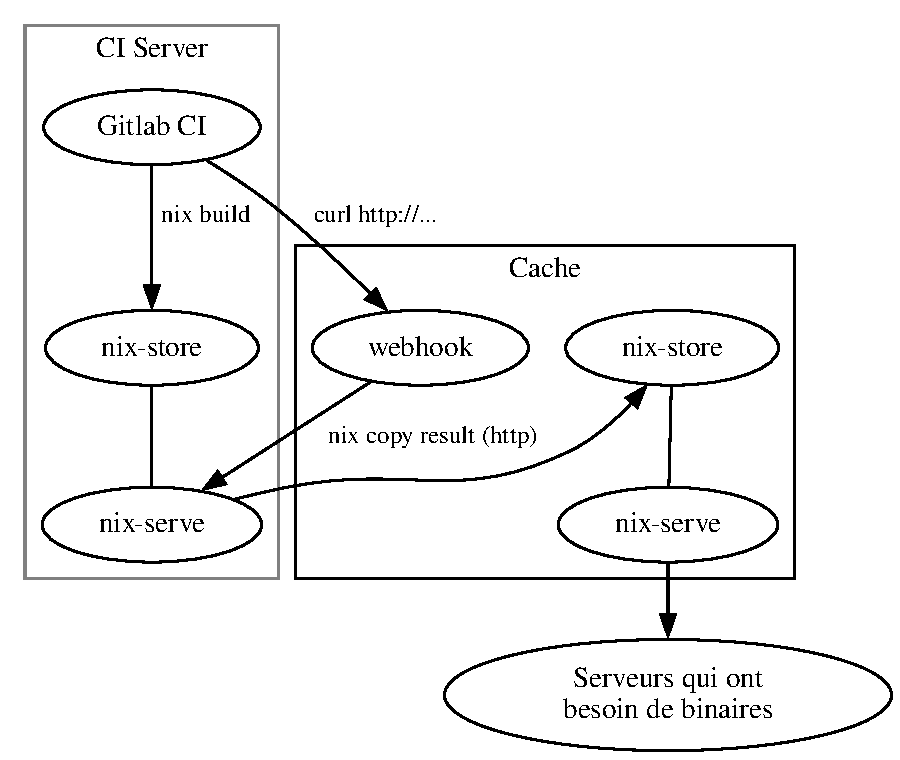
\includegraphics[width=10cm]{./media/ci.pdf}
	\caption{Schéma de principe du cache}\label{fig:ci}
\end{figure}

Le principe est simple. Le runner de la CI va compiler les paquets nécessaires
(par exemple via la commande \texttt{nix build}) puis va faire un requête au webhook
http du serveur de cache. Cette requête contient des données sur le
\emph{store-path} à enregistrer dans le cache. En particulier elle contient:
\begin{itemize}
	\item Le chemin du \emph{store-path} à sauver
	\item Le hash du commit
	\item La date du commit
\end{itemize}

En recevant la requête, le serveur de cache va télécharger la dérivation puis
créer un lien symbolique vers celle-ci à l'emplacement
\url{/nix/var/nix/gcroots/cacheroots/[NOM\_DU\_PROJET\_GIT]/[NOM\_DE\_BRANCHE]/[HASH\_DU\_COMMIT]}.
Ce téléchargement se fait grace au programme \texttt{nix-store} qui sert le
store du \emph{runner} en HTTP.\@

J'ai développé ensuite un script en ligne de commande qui permet de gerer les
liens symboliques ainsi créés. En particulier:
\begin{itemize}
	\item Il liste les différents commits sauvegardés d'un dépot/d'une bran
		branche avec les messages de commit
	\item Il aide à supprimer les liens symboliques avec une politique
		précise (les $n$ derniers par branche ou les commits antérieurs à
		une certaine date)
	\item Il vérifie que le données sauvegardées (date du commit, branche,
		etc) sont correctes. Il ne vérifie pas cependant que le couple
		(hash du commit, \emph{store-path}) est correct car cela coûte
		une évaluation \texttt{nix} et il n'est pas prévu d'effectuer
		des évaluations sur la machine de cache (évaluations qui peuvent
		parfois demander un montant non négligeable de plusieurs
		giga-octets de RAM et peuvent être assez longues).

\end{itemize}

\subsection*{Sécurité}

On considère que le contenu des dérivations \emph{nix} n'est jamais secret. En effet,
le \emph{store} est lisible par tout le monde sur la machine et dans notre cas,
le store entier est servi en HTTP via le programme \texttt{nix-serve}.

De plus, le webhook fait confiance aux informations fournies pour le client sur
le commit à sauver. Le script exécuté par le webhook pourrait faire certaines
vérifications mais je ne les ai pas implémentées. A priori la vérification la
plus couteuse serait de vérifier que la dérivation correspond bien au hash du
commit (elle coûte une évaluation \emph{nix}, mais pas une instanciation). Pour
rendre plus complexe la compromission de cette paire, le webhook implémente une
liste d'accès bassée sur l'ip du client.

Enfin, le mécanisme de signature du store de nixos fait  que le contenu des
paquets ne sera jamais compromis.

En résumé un attaquant ayant accès au réseau entre le \emph{runner} et le cache
peut faire sauvegarder des dérivations en trop mais ne peut pas compromettre le
contenu des paquets (qui lui est protégé par des mécanismes internes à
\emph{nix}).


\section{Les tailles des closures}

La dernière tâche de mon stage à été d'essayer d'estimer la taille des paquets à
sauvegarder afin de dimensionner le serveur de cache. Cette tâche n'était pas
vraiment facile étant donnée que encore peu de paquets étaient développés
pendant mon stage.

J'ai principalement essayé d'évaluer l'espace occupé par les dépendances de
compilation du paquet \texttt{hello} selon la révision de
\emph{nixpkgs}\footnote{\emph{nixpkgs} est une grande expression \emph{nix}
contenant beaucoup de programmes différents.} utilisée
et surtout de repérer les changements de dépendances.

Mon travail n'a été que partiel car j'ai évalué les résultats seulement sur un
nombre restreint de révisions étalées régulièrement dans le temps. Pour cela
j'ai utilisé un méthode naïve consistant à instancier toutes les version
différentes (et donc de tout télécharger). Il est évident que j'aurais dû écrire
un script qui évalue la taille des \emph{store-paths} en utilisant les
meta-données présentes sur \url{https://cache.nixos.org}.

Les résultats sont les suivants:


Sur 26 révisions de \emph{nixpkgs}, on observe 6 modifications notables de
\emph{stdenv}\footnote{\emph{stdenv} est la dérivation contenant la toolchain
C/C++ standard de nix}. Ces modifications consistent en l'ajout de patchs. Les
sources restent identiquent.

En terme d'espace, la clôture complète de \emph{gnu-hello} est d'un peu moins de
2Go. Les 26 versions de hello ainsi compilées prennent un total de
$\SI{17.2}{\gibi\byte}$. Cette taille ne prend pas en compte la déduplication
expliquée au paragraphe suivant mais fais bien ganger de l'espace du fait de
dépendances qui sont égales.

Il faut bien noter que \emph{nix} possède d'autres optimisations pour l'espace
de stockage, notamment il implémente un système de déduplication des fichiers
avec du hard-linking (rendu possible par le carractère immutable du contenu
des \emph{store-paths}).

J'ai évalué aussi la taille du framework C utilisé pour le contrôle commande
(EPICS) accompagné des différents clients pour les opérateurs des accélérateurs.
La clôture étendue de l'ensembles des paquets packagés dans EPNix~\cite{epnix} (la version
``nixifiée'' de EPICS) fait $\SI{18}{\gibi\byte}$.

\section{Conclusion}

Mon stage mis en évidence la difficulté à référencer l'ensemble des dépendances
de compilation avec nix. Il a aussi permis au labo d'obtenir des expressions
nixos pour le cache et mettre en place un système de gestion des résultats de
build avec la CI.\@

\subsection*{Bilan personnel}

Ce stage m'a aussi fait découvrir comment fonctionne la construction d'un
accélérateur et ça m'a permi de satisfaire en partie ma curiosité sur tous les
éléments périphériques d'un accélérateur (protection des rédiation, commande,
acquisition,\dots).

De plus, j'ai apprécié être au contact d'ingénieurs et de se confronter à des
problématiques plus concrètes (résoudre un problème avec un objectif clair).

Finalement, j'ai beaucoup aimé l'ambiance dans le labo. Je remercie beaucoup mon
tuteur \nom{Remi}{Nicole} qui m'a encadré tout au long du stage.

\printbibliography{}

\end{document}
